\section{Three-level system}\label{sec:pw3l}

A two-level system is the simplest non-trivial quantum system and,
as seen in Sec.~\ref{sec:absorption+pw},
it is sufficient to illustrate
models of quantum time of arrival
such as those based on complex potentials,
as well as relational models.
Therein, numerical examples have been shown where the two approaches
---discrete Page--Wootters and the ``non Hermitian'' detector models---
lead to
compatible predictions.

A three-level atom (or a three-level quantum system in general) \emph{may} appear as
the next natural step, by studying a system at the immediately further
degree of complexity, but otherwise showing essentially
the same physics. In fact, there are more practical and conceptual reasons
for an interest in three-level systems specifically; and a phenomenology
that can only be shown in a system with three energy levels or more.

\subsection{Lit}
\cite{Ruschhaupt_AtomDiode} -- Improvement by laser quenching of an `atom diode': a one-way barrier for ultra-cold atoms.

\cite{NonHermitianShortcutSTIRAP} -- Non-Hermitian shortcut to stimulated Raman adiabatic passage.

\cite{EIT_Review} -- Electromagnetically induced transparency: Optics in coherent media.

\cite{OptimizedTransferSTIRAP} -- Optimized three-level quantum transfers based on frequency-modulated optical excitations


\subsection{Figures}

Lorem ipsum.

% \begin{figure}
%   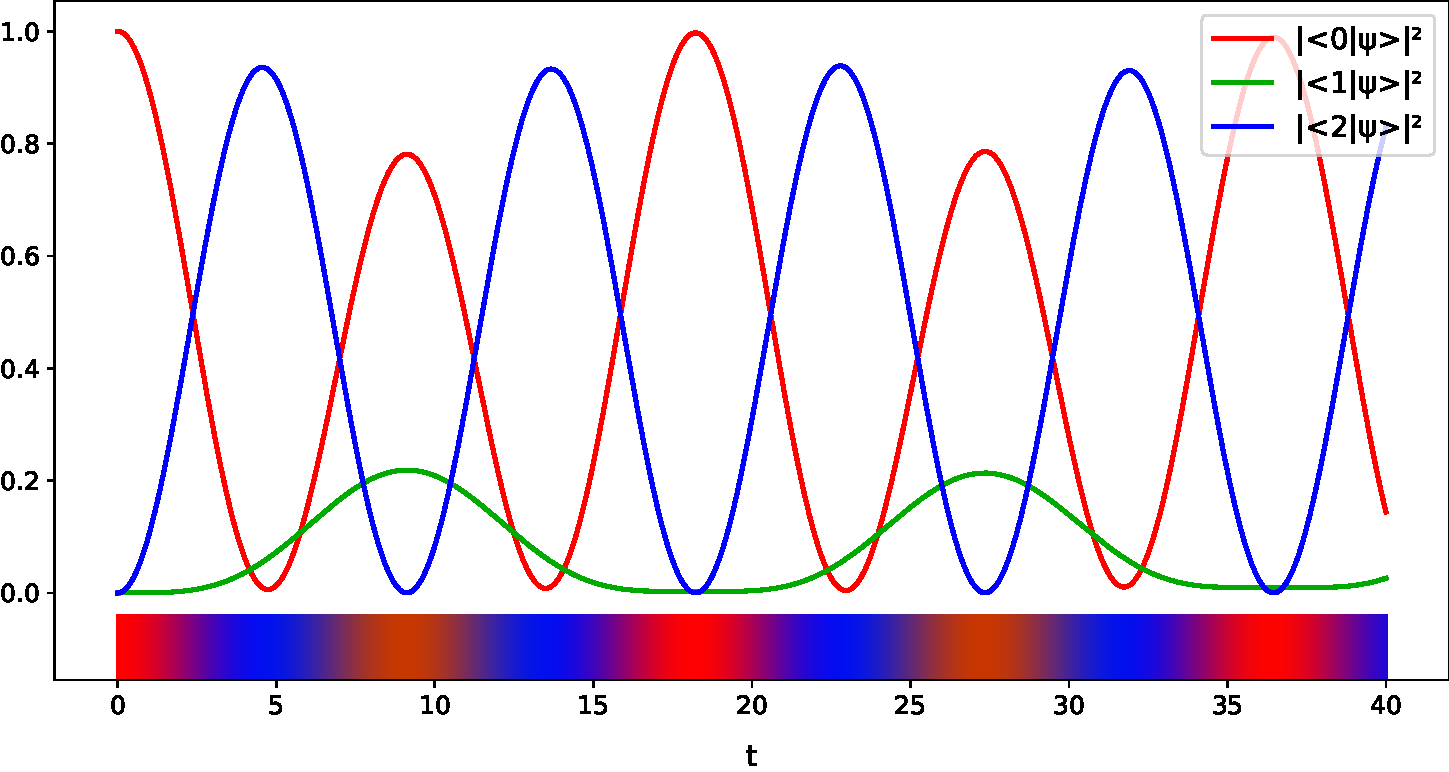
\includegraphics[width=\textwidth]{img/3ldetect/hermitian3lines.pdf}
%   \caption{Foobar.}
%   %\label{fig:psi_V}
% \end{figure}

% \begin{figure}
%   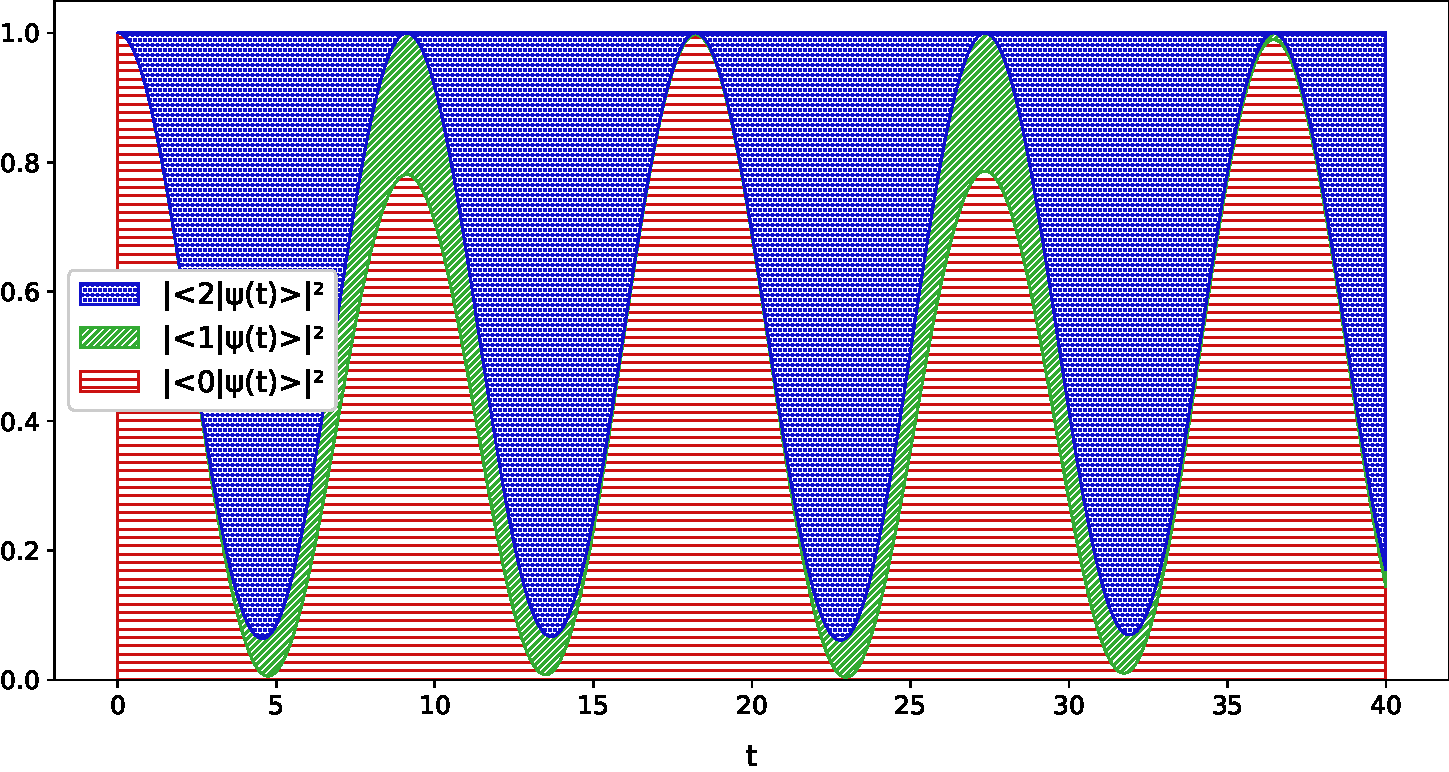
\includegraphics[width=\textwidth]{img/3ldetect/hermitian3color.pdf}
%   \caption{Fooboo.}
%   %\label{fig:psi_V}
% \end{figure}

\begin{figure}[h]
  \centering
  \begin{subfigure}[b]{\textwidth}
    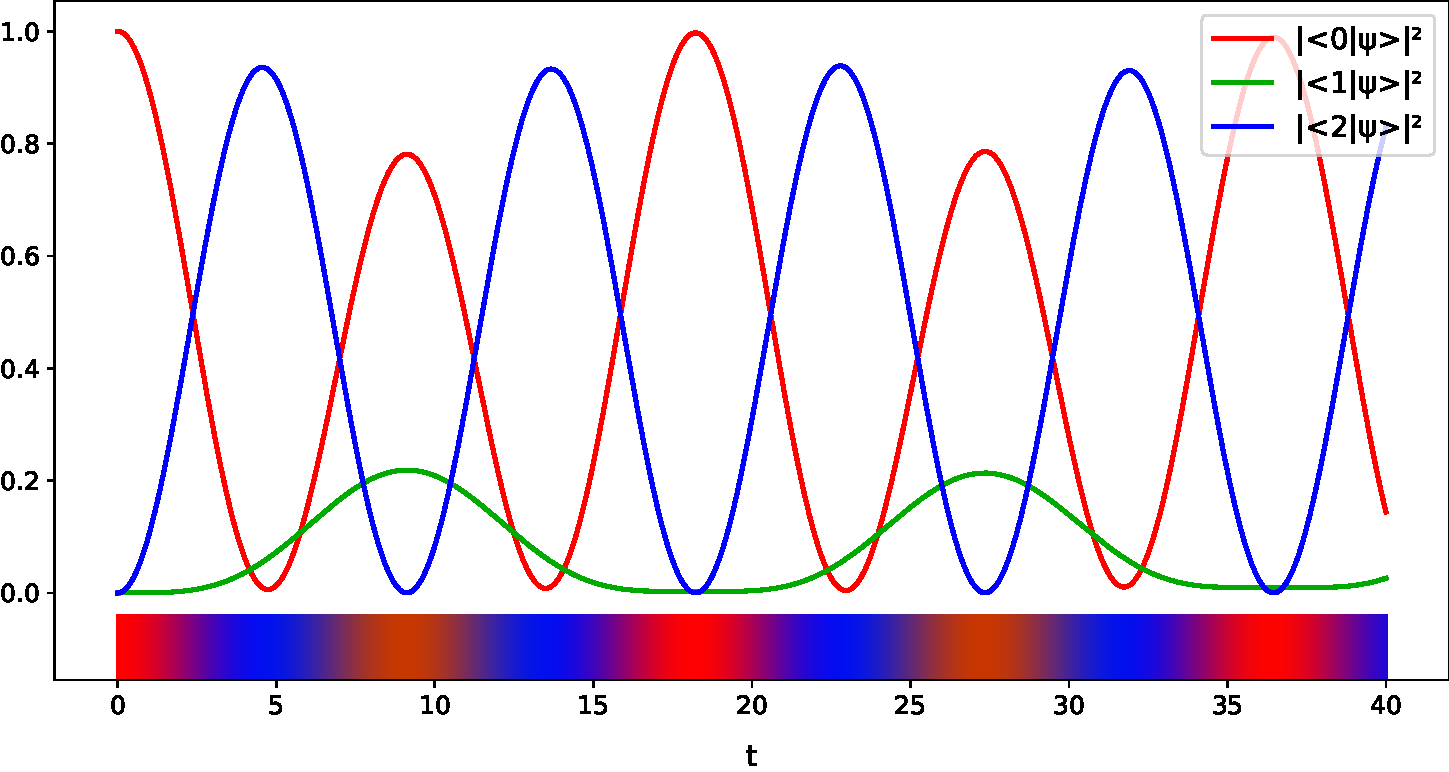
\includegraphics[width=\textwidth]{img/3ldetect/hermitian3lines.pdf}
    \subcaption{Foo.}%\label{fig:aabsorbed-qubit-components_pwlattice:re0}
  \end{subfigure}
  \par\bigskip
  \par\bigskip
  \begin{subfigure}[b]{\textwidth}
    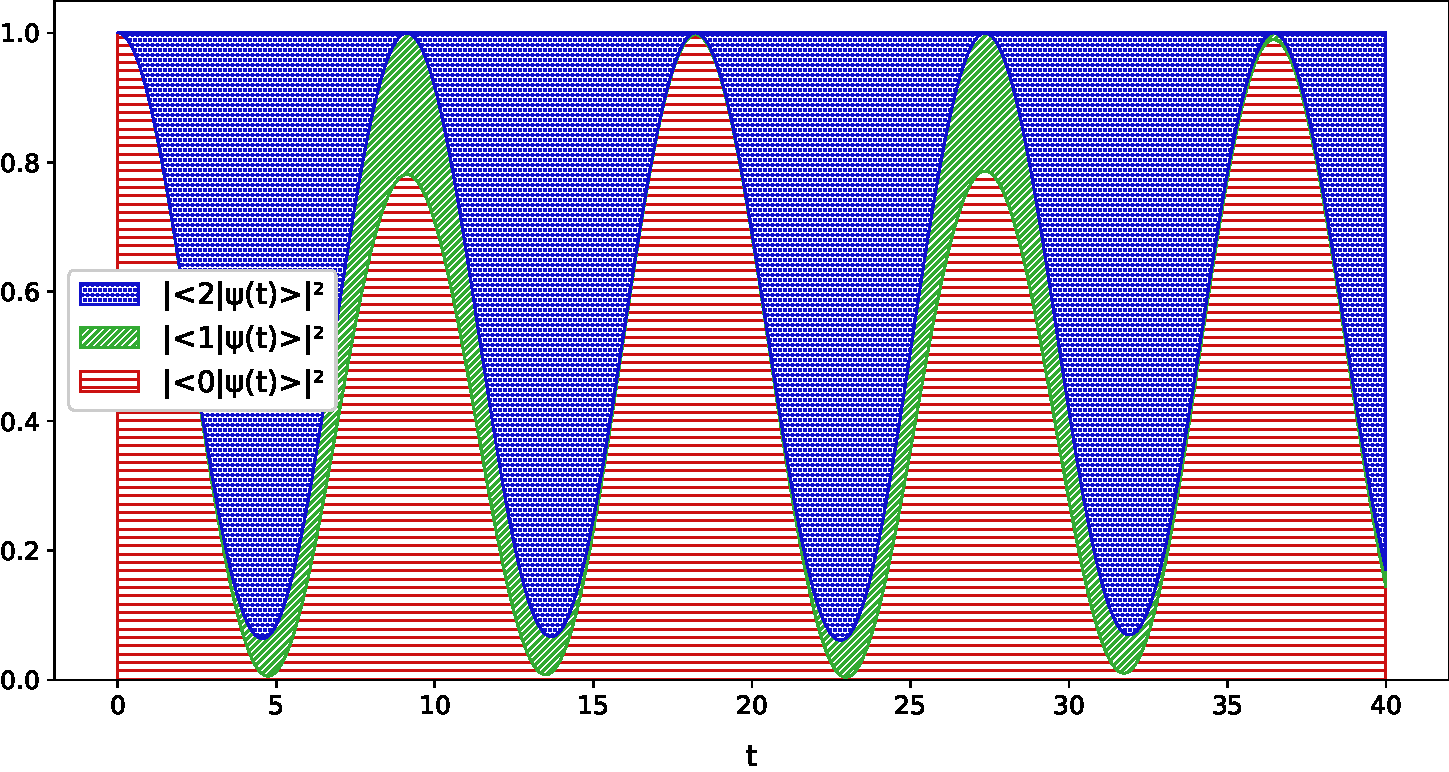
\includegraphics[width=\textwidth]{img/3ldetect/hermitian3color.pdf}
    \subcaption{Bar.}%\label{fig:aabsorbed-qubit-components_pwlattice:im1}
  \end{subfigure}
  \par\bigskip
  \par\bigskip
  \caption{
    Blah blah blah.
  }
  \label{fig:aabsorbed-qubit-components_pwlattice}
\end{figure}

% \begin{figure}[hb!]
%   \centering
%   \begin{subfigure}{\textwidth}
%       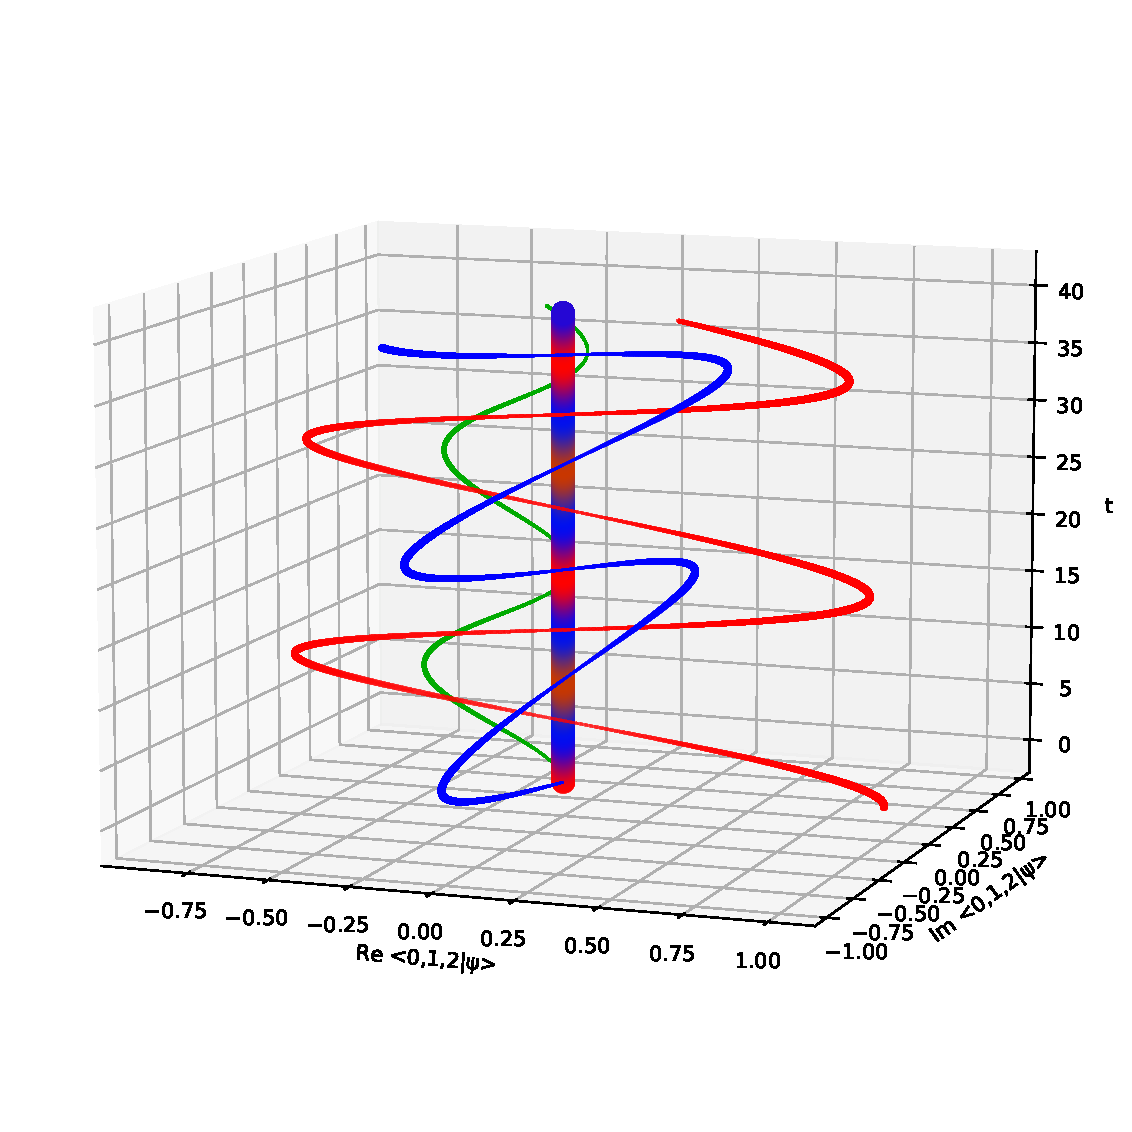
\includegraphics[width=\textwidth]{img/3ldetect/hermitianSpaceTime_side.pdf}
%       \subcaption{Foo.}
%       %\label{fig:arm1}
%   \end{subfigure}
%   \caption{Foobar.}
% \end{figure}%
% \begin{figure}[ht]\ContinuedFloat
%   \centering
%   \begin{subfigure}{\textwidth}
%       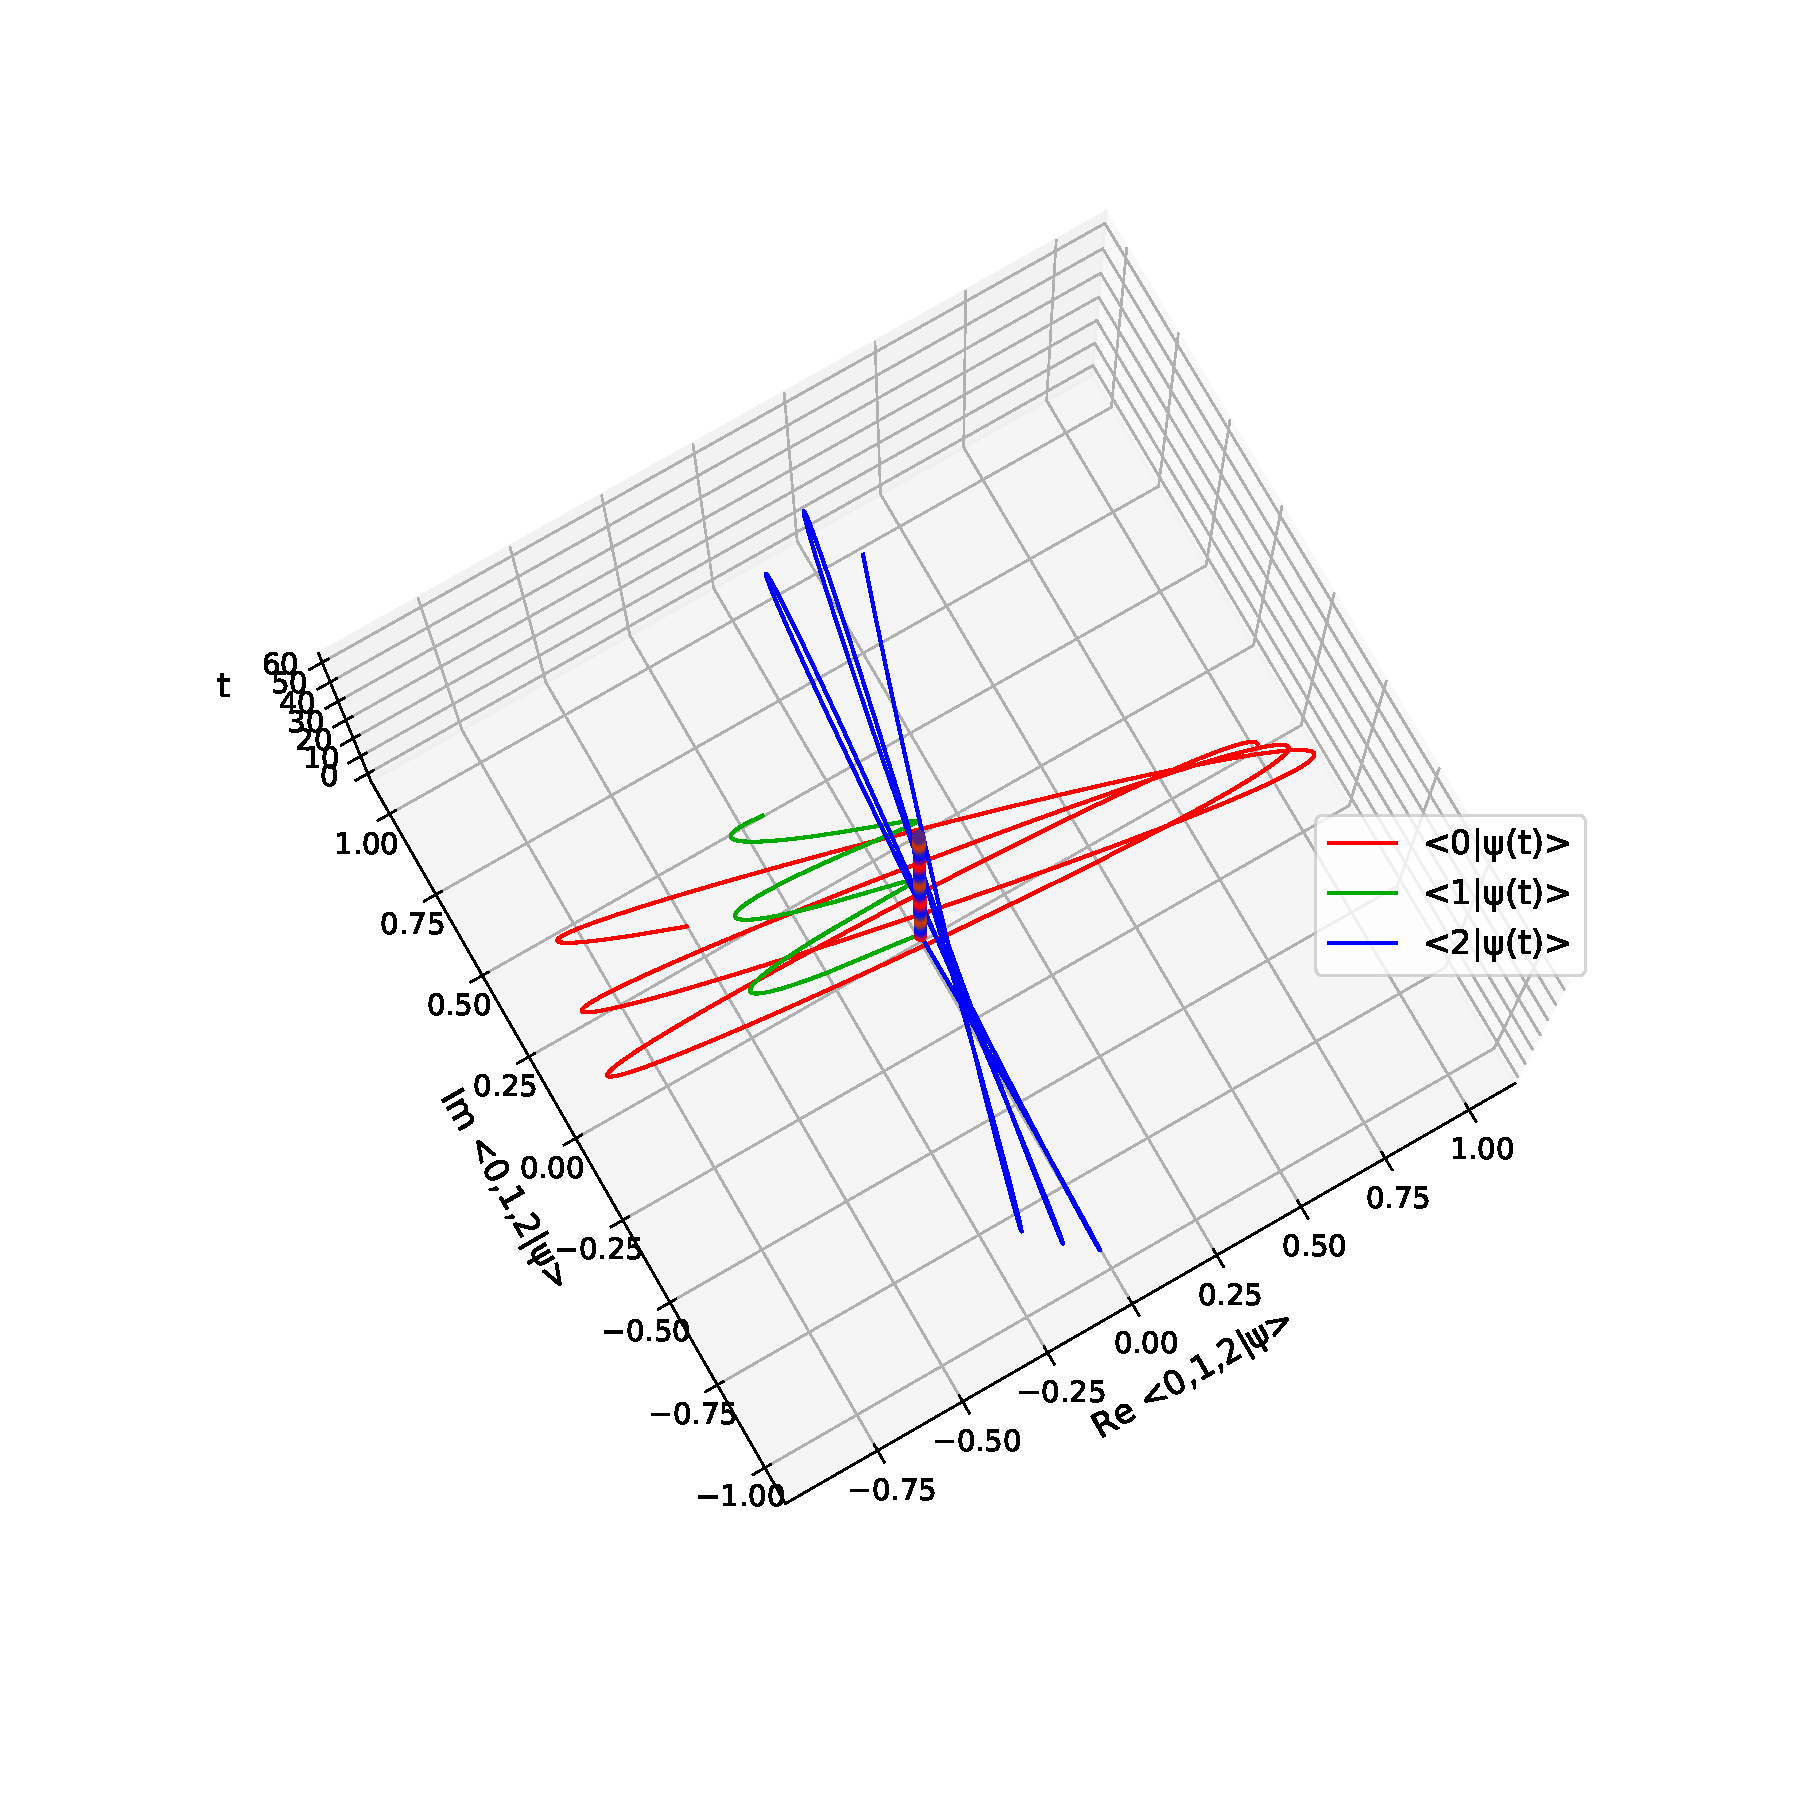
\includegraphics[width=\textwidth]{img/3ldetect/hermitianSpaceTime_top.pdf}
%       \subcaption{Bar.}
%       %\label{fig:arm3}
%   \end{subfigure}
%   \caption{Foobar (cont.)}
% \end{figure}


\begin{figure}
  \centering
  \begin{subfigure}[b]{\textwidth}
    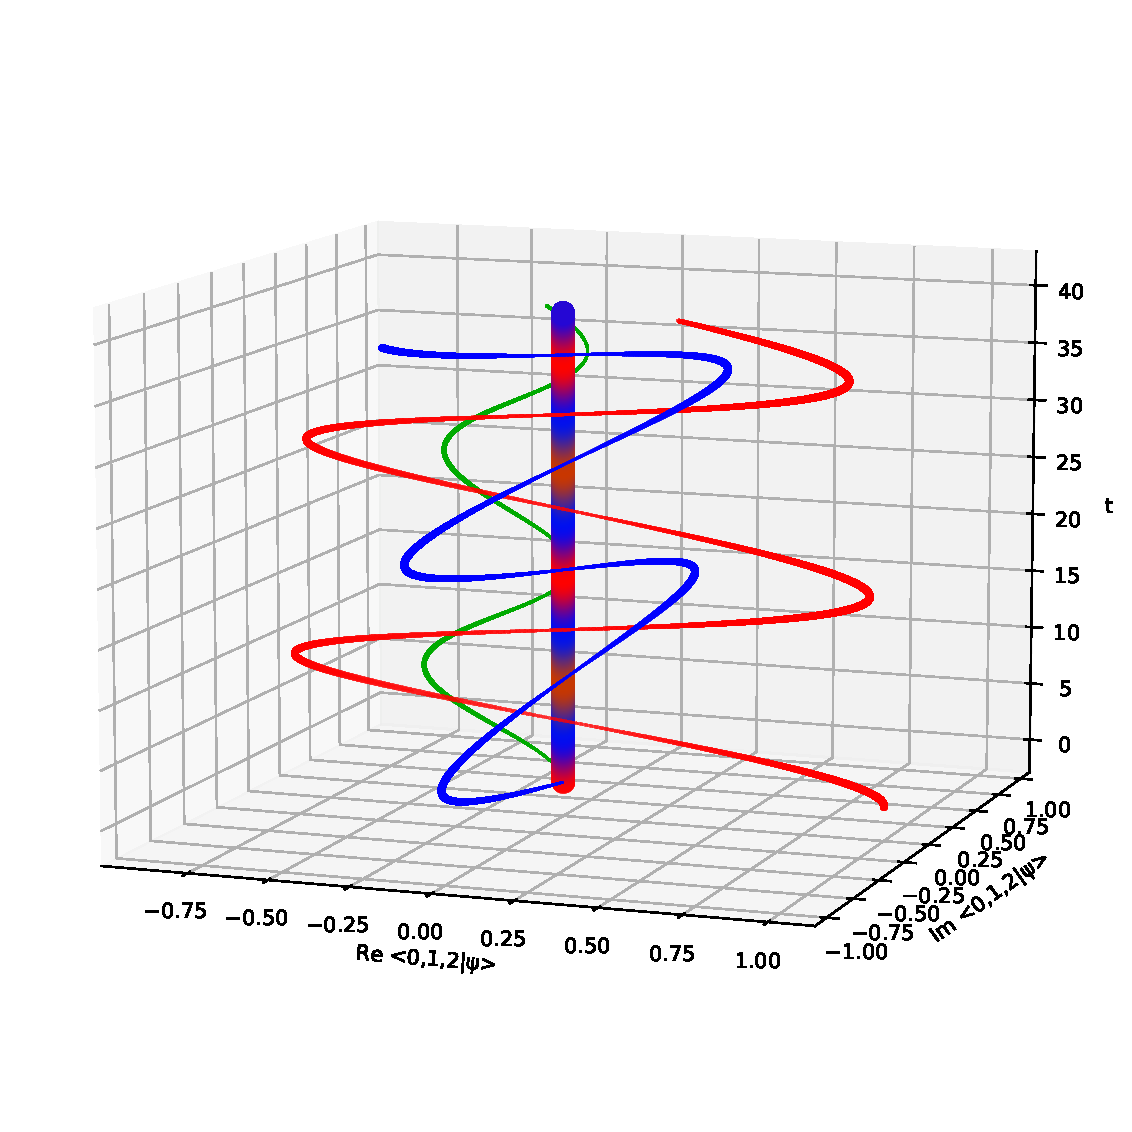
\includegraphics[height=0.4\textheight,clip,trim=60 80 0 120]{img/3ldetect/hermitianSpaceTime_side.pdf}
    \caption{Foo.}
  \end{subfigure}
  \par\bigskip
  \begin{subfigure}[b]{\textwidth}
    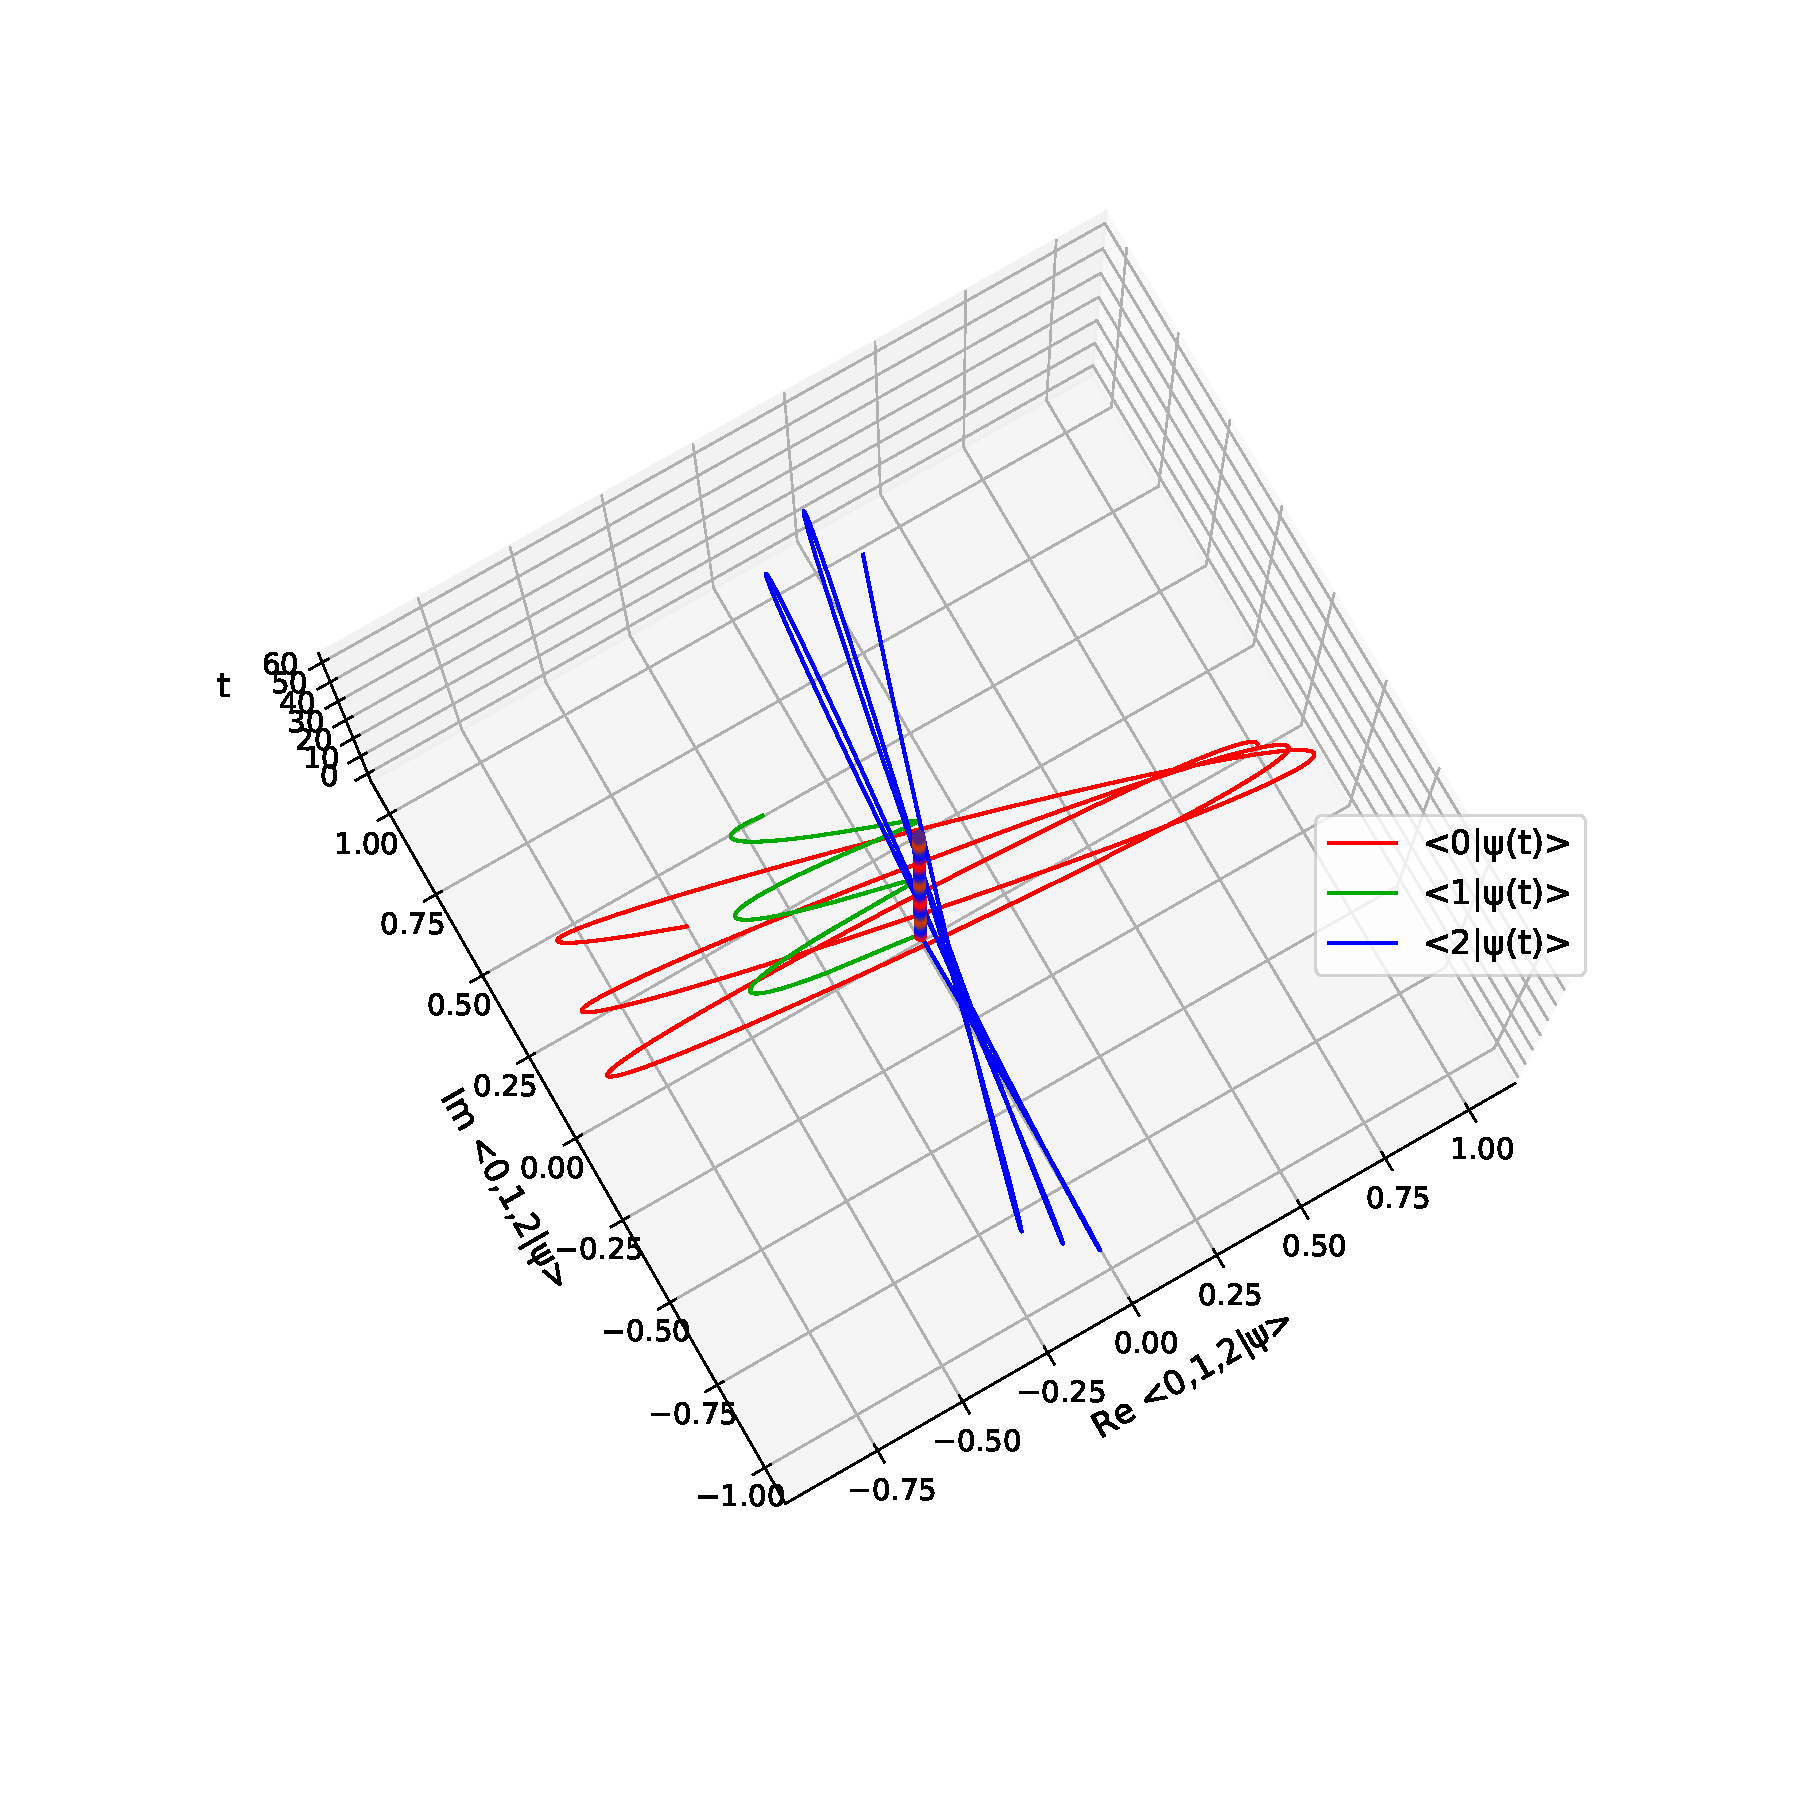
\includegraphics[height=0.5\textheight,clip,trim= 0 20 0 80]{img/3ldetect/hermitianSpaceTime_top.pdf}
    \caption{Bar.}
  \end{subfigure}
  \par\bigskip
  \caption{FooBar.}
  %\label{fig:psi_V}
\end{figure}

% \begin{figure}
%   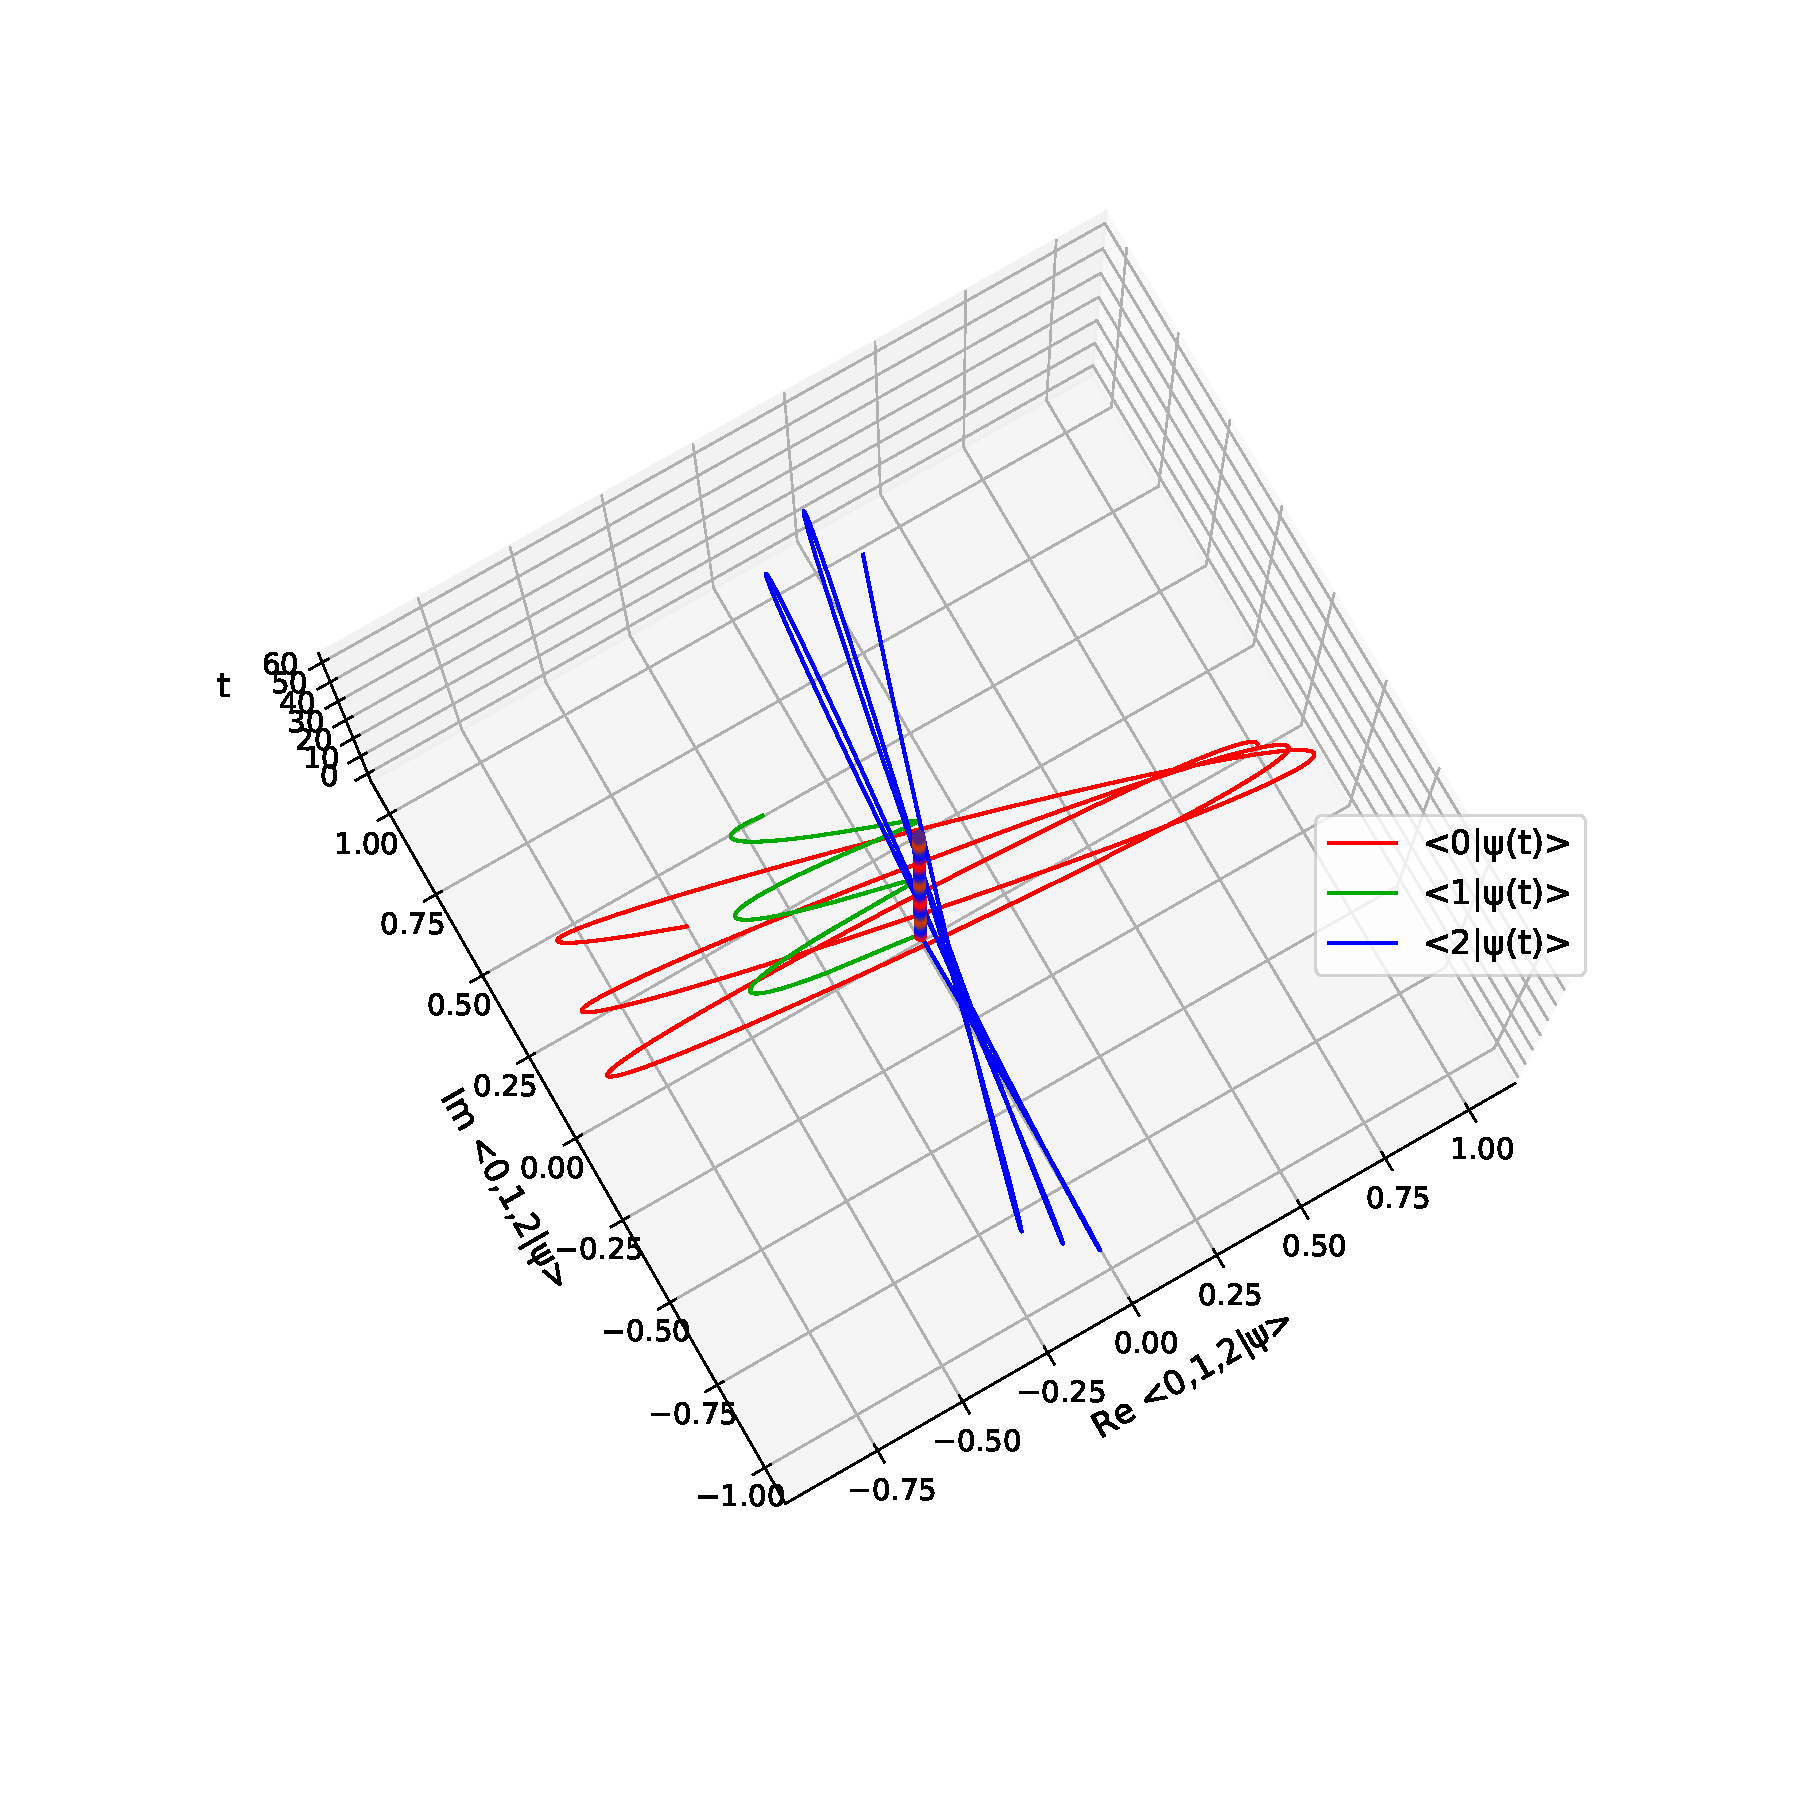
\includegraphics[width=\textwidth]{img/3ldetect/hermitianSpaceTime_top.pdf}
%   \caption{Bar.}
%   %\label{fig:psi_V}
% \end{figure}

% \begin{figure}
%   \centering
%   \begin{subfigure}[b]{1.0\textwidth}
%     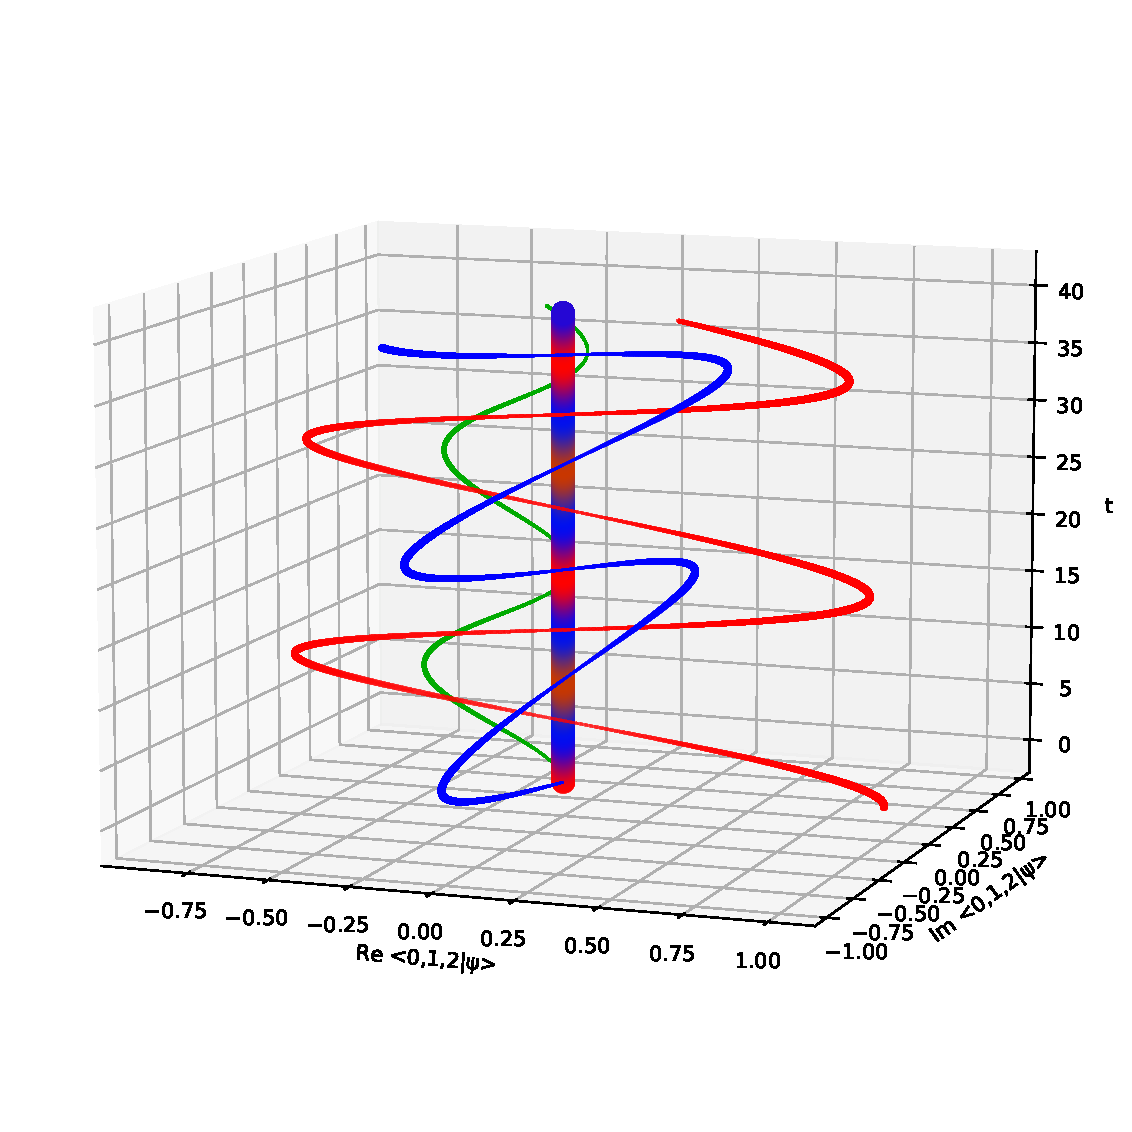
\includegraphics[height=0.5\textheight]{img/3ldetect/hermitianSpaceTime_side.pdf}
%     \subcaption{Foo.}%\label{fig:aabsorbed-qubit-components_pwlattice:re0}
%   \end{subfigure}\\
%   \begin{subfigure}[b]{1.0\textwidth}
%     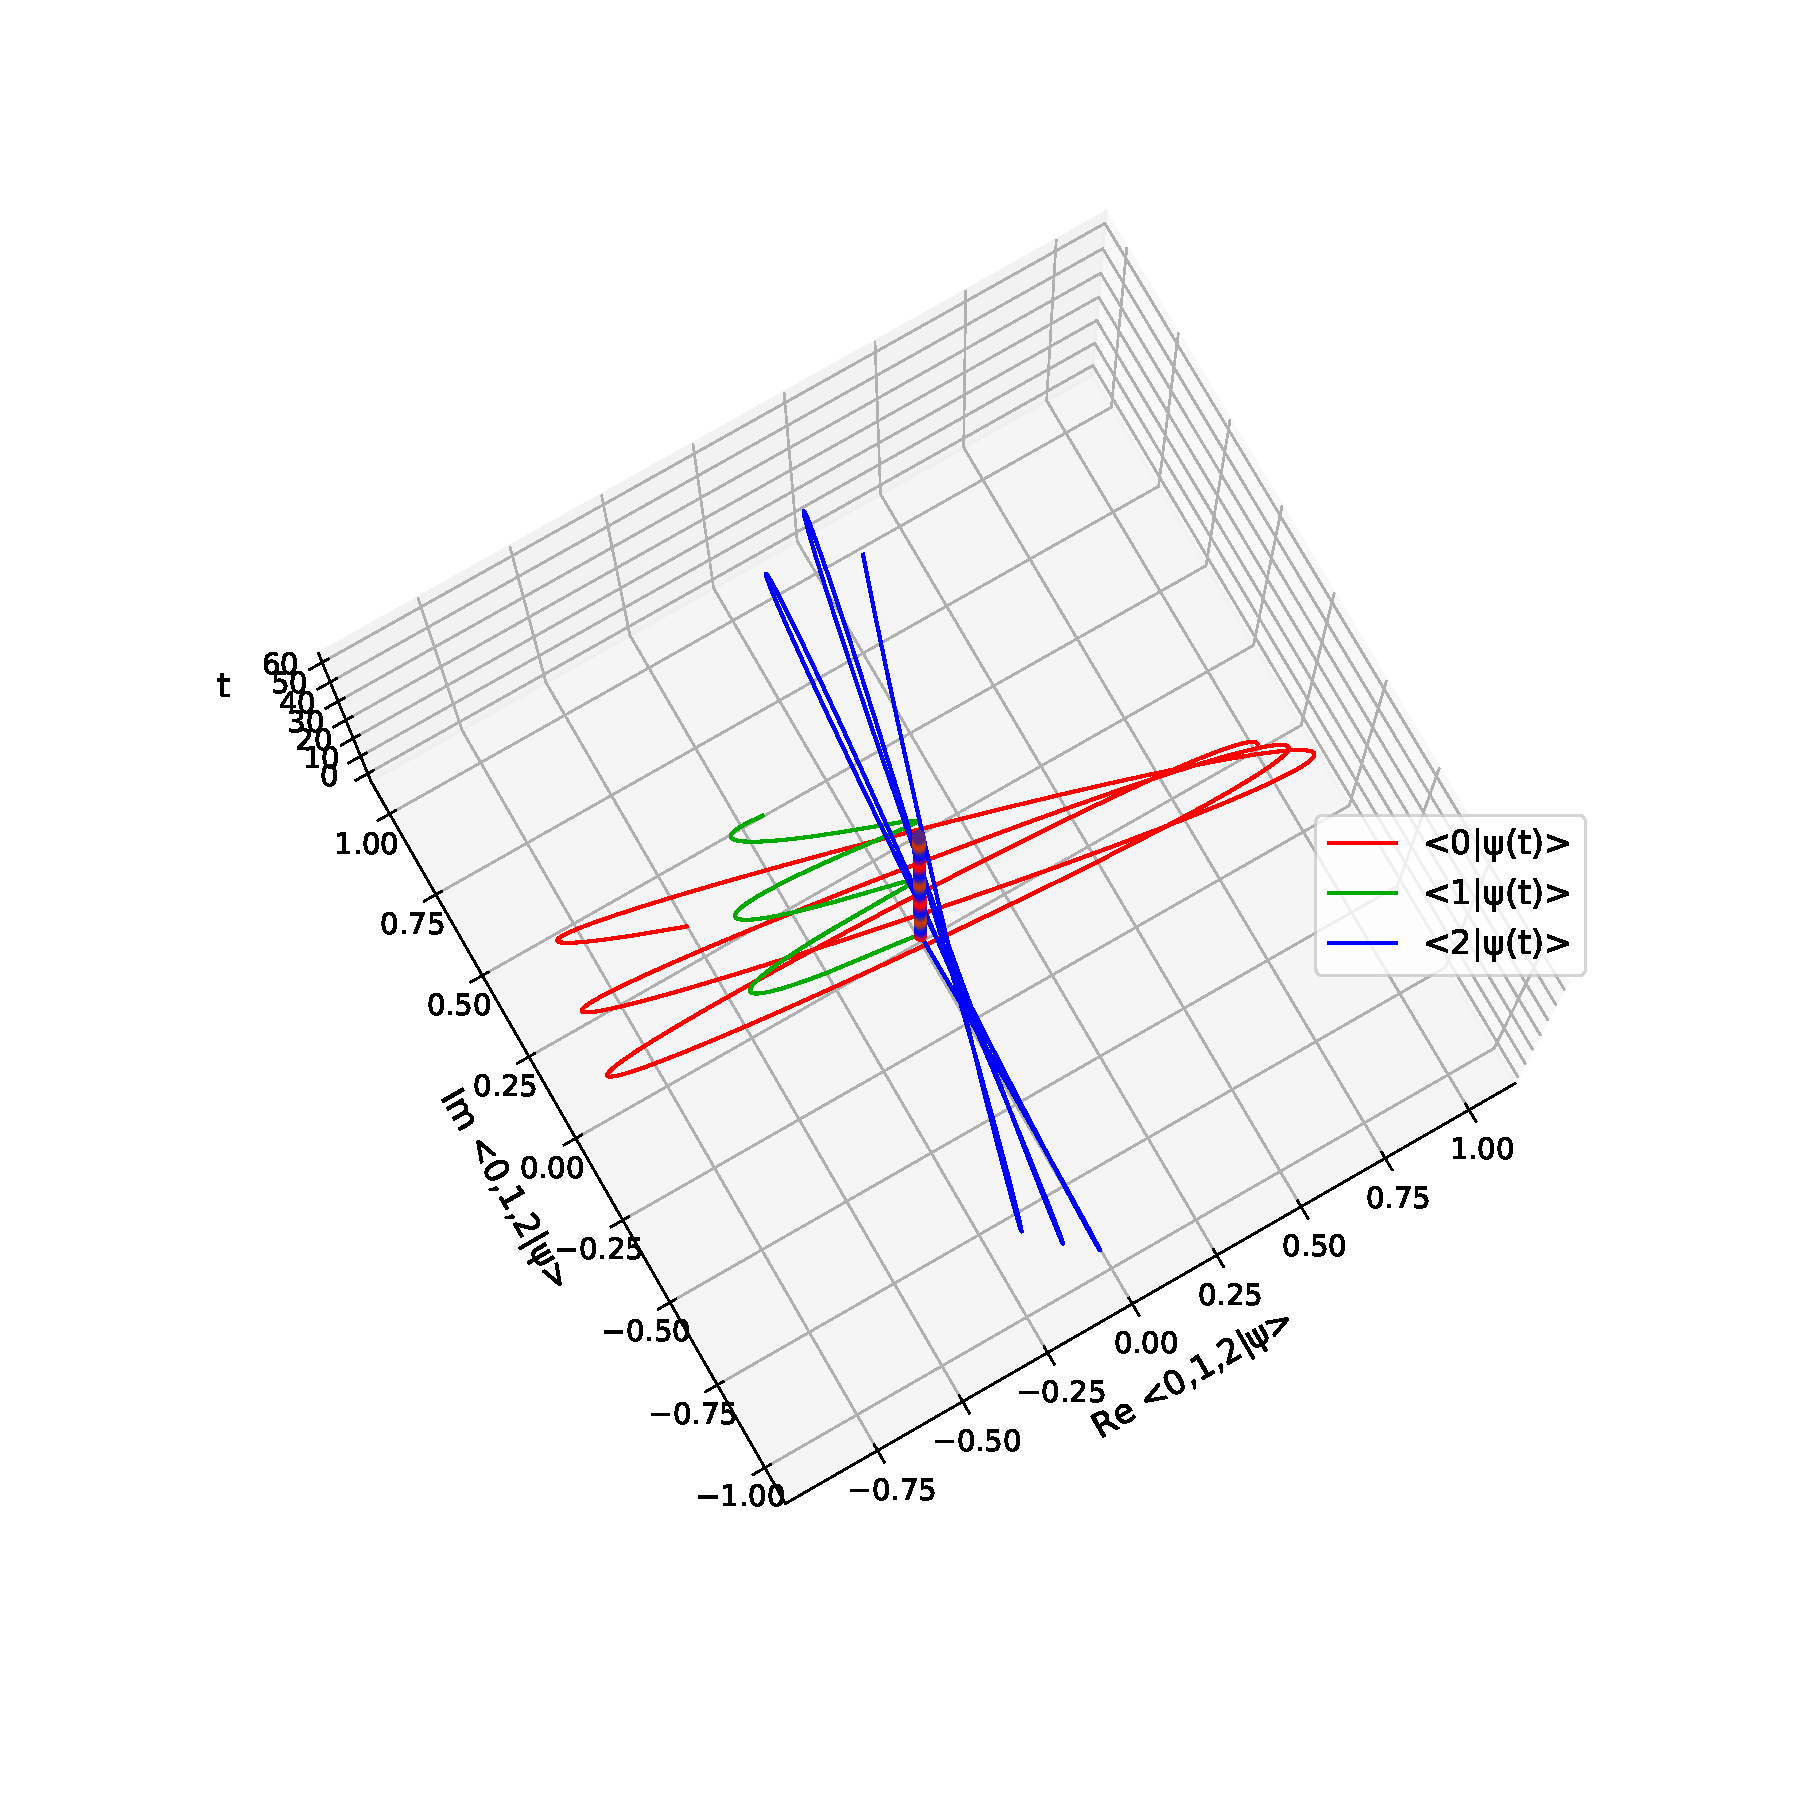
\includegraphics[height=0.5\textheight]{img/3ldetect/hermitianSpaceTime_top.pdf}
%     \subcaption{Bar.}\label{fig:aabsorbed-qubit-components_pwlattice:im1}
%   \end{subfigure}
%   \caption{
%     Blah blah blah.
%   }
%   \label{fig:aabsorbed-qubit-components_pwlattice}
% \end{figure}
